% AUTO-GENERATED by paper/tools/export_results.py (TikZ; teacher means over the 3 new draws;
% Pop/Pop uses no calibration draw). Colours: validated categorical slots 1-2.
\definecolor{unifc}{HTML}{2A78D6}
\definecolor{minic}{HTML}{EB6834}
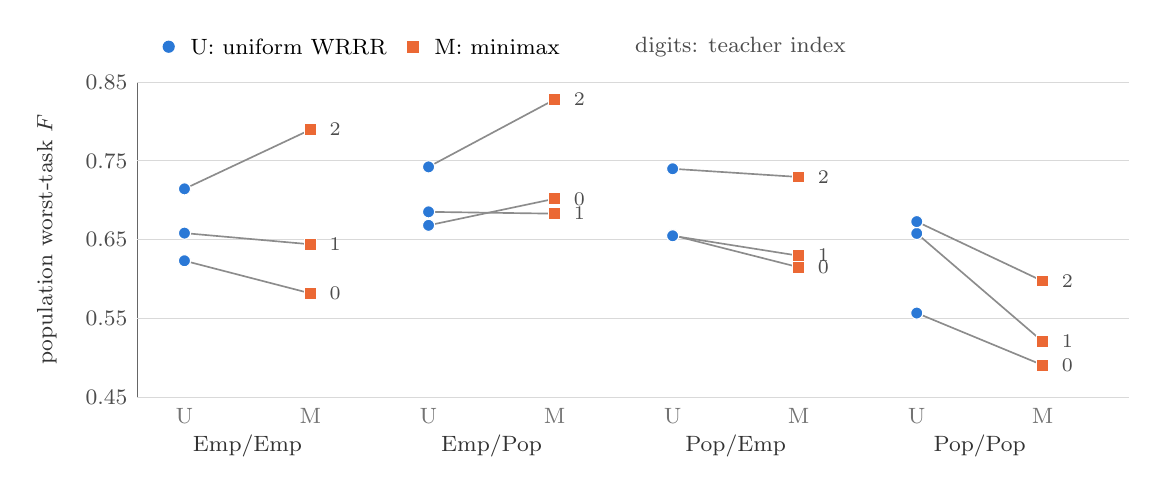
\begin{tikzpicture}[x=1cm,y=1cm,font=\footnotesize]
\draw[black!60] (0,0) -- (0,4.000);
\draw[black!15] (0,0.000) -- (12.6,0.000);
\node[anchor=east,text=black!70] at (0,0.000) {0.45};
\draw[black!15] (0,1.000) -- (12.6,1.000);
\node[anchor=east,text=black!70] at (0,1.000) {0.55};
\draw[black!15] (0,2.000) -- (12.6,2.000);
\node[anchor=east,text=black!70] at (0,2.000) {0.65};
\draw[black!15] (0,3.000) -- (12.6,3.000);
\node[anchor=east,text=black!70] at (0,3.000) {0.75};
\draw[black!15] (0,4.000) -- (12.6,4.000);
\node[anchor=east,text=black!70] at (0,4.000) {0.85};
\node[rotate=90,anchor=south,text=black!80] at (-0.9,2.000) {population worst-task $F$};
\node[anchor=north,text=black!80] at (1.40,-0.35) {Emp/Emp};
\node[anchor=north,text=black!55] at (0.60,-0.02) {U};
\node[anchor=north,text=black!55] at (2.20,-0.02) {M};
\draw[black!45,line width=0.6pt] (0.60,1.732) -- (2.20,1.318);
\fill[unifc,draw=white,line width=0.4pt] (0.60,1.732) circle (2.2pt);
\fill[minic,draw=white,line width=0.4pt] (2.125,1.243) rectangle (2.275,1.393);
\node[anchor=west,text=black!70,font=\scriptsize] at (2.32,1.318) {0};
\draw[black!45,line width=0.6pt] (0.60,2.083) -- (2.20,1.941);
\fill[unifc,draw=white,line width=0.4pt] (0.60,2.083) circle (2.2pt);
\fill[minic,draw=white,line width=0.4pt] (2.125,1.866) rectangle (2.275,2.016);
\node[anchor=west,text=black!70,font=\scriptsize] at (2.32,1.941) {1};
\draw[black!45,line width=0.6pt] (0.60,2.645) -- (2.20,3.397);
\fill[unifc,draw=white,line width=0.4pt] (0.60,2.645) circle (2.2pt);
\fill[minic,draw=white,line width=0.4pt] (2.125,3.322) rectangle (2.275,3.472);
\node[anchor=west,text=black!70,font=\scriptsize] at (2.32,3.397) {2};
\node[anchor=north,text=black!80] at (4.50,-0.35) {Emp/Pop};
\node[anchor=north,text=black!55] at (3.70,-0.02) {U};
\node[anchor=north,text=black!55] at (5.30,-0.02) {M};
\draw[black!45,line width=0.6pt] (3.70,2.182) -- (5.30,2.519);
\fill[unifc,draw=white,line width=0.4pt] (3.70,2.182) circle (2.2pt);
\fill[minic,draw=white,line width=0.4pt] (5.225,2.444) rectangle (5.375,2.594);
\node[anchor=west,text=black!70,font=\scriptsize] at (5.42,2.519) {0};
\draw[black!45,line width=0.6pt] (3.70,2.353) -- (5.30,2.330);
\fill[unifc,draw=white,line width=0.4pt] (3.70,2.353) circle (2.2pt);
\fill[minic,draw=white,line width=0.4pt] (5.225,2.255) rectangle (5.375,2.405);
\node[anchor=west,text=black!70,font=\scriptsize] at (5.42,2.330) {1};
\draw[black!45,line width=0.6pt] (3.70,2.924) -- (5.30,3.779);
\fill[unifc,draw=white,line width=0.4pt] (3.70,2.924) circle (2.2pt);
\fill[minic,draw=white,line width=0.4pt] (5.225,3.704) rectangle (5.375,3.854);
\node[anchor=west,text=black!70,font=\scriptsize] at (5.42,3.779) {2};
\node[anchor=north,text=black!80] at (7.60,-0.35) {Pop/Emp};
\node[anchor=north,text=black!55] at (6.80,-0.02) {U};
\node[anchor=north,text=black!55] at (8.40,-0.02) {M};
\draw[black!45,line width=0.6pt] (6.80,2.056) -- (8.40,1.650);
\fill[unifc,draw=white,line width=0.4pt] (6.80,2.056) circle (2.2pt);
\fill[minic,draw=white,line width=0.4pt] (8.325,1.575) rectangle (8.475,1.725);
\node[anchor=west,text=black!70,font=\scriptsize] at (8.52,1.650) {0};
\draw[black!45,line width=0.6pt] (6.80,2.049) -- (8.40,1.796);
\fill[unifc,draw=white,line width=0.4pt] (6.80,2.049) circle (2.2pt);
\fill[minic,draw=white,line width=0.4pt] (8.325,1.721) rectangle (8.475,1.871);
\node[anchor=west,text=black!70,font=\scriptsize] at (8.52,1.796) {1};
\draw[black!45,line width=0.6pt] (6.80,2.900) -- (8.40,2.796);
\fill[unifc,draw=white,line width=0.4pt] (6.80,2.900) circle (2.2pt);
\fill[minic,draw=white,line width=0.4pt] (8.325,2.721) rectangle (8.475,2.871);
\node[anchor=west,text=black!70,font=\scriptsize] at (8.52,2.796) {2};
\node[anchor=north,text=black!80] at (10.70,-0.35) {Pop/Pop};
\node[anchor=north,text=black!55] at (9.90,-0.02) {U};
\node[anchor=north,text=black!55] at (11.50,-0.02) {M};
\draw[black!45,line width=0.6pt] (9.90,1.068) -- (11.50,0.406);
\fill[unifc,draw=white,line width=0.4pt] (9.90,1.068) circle (2.2pt);
\fill[minic,draw=white,line width=0.4pt] (11.425,0.331) rectangle (11.575,0.481);
\node[anchor=west,text=black!70,font=\scriptsize] at (11.62,0.406) {0};
\draw[black!45,line width=0.6pt] (9.90,2.079) -- (11.50,0.705);
\fill[unifc,draw=white,line width=0.4pt] (9.90,2.079) circle (2.2pt);
\fill[minic,draw=white,line width=0.4pt] (11.425,0.630) rectangle (11.575,0.780);
\node[anchor=west,text=black!70,font=\scriptsize] at (11.62,0.705) {1};
\draw[black!45,line width=0.6pt] (9.90,2.229) -- (11.50,1.473);
\fill[unifc,draw=white,line width=0.4pt] (9.90,2.229) circle (2.2pt);
\fill[minic,draw=white,line width=0.4pt] (11.425,1.398) rectangle (11.575,1.548);
\node[anchor=west,text=black!70,font=\scriptsize] at (11.62,1.473) {2};
\fill[unifc] (0.4,4.450) circle (2.2pt);
\node[anchor=west] at (0.55,4.450) {U: uniform WRRR};
\fill[minic] (3.425,4.375) rectangle (3.575,4.525);
\node[anchor=west] at (3.65,4.450) {M: minimax};
\node[anchor=west,text=black!70] at (6.2,4.450) {digits: teacher index};
\end{tikzpicture}
